\chapter[INTRODUÇÃO]{INTRODUÇÃO}



\begin{itemize}
 \item para inserir uma sigla: 
    \verb|\criarsigla|\{ABNT\}{Associa\c{c}\~ao Brasileira de Normas T\'ecnicas}:

    \criarsigla{ABNT}{Associa\c{c}\~ao Brasileira de Normas T\'ecnicas}

\item para inserir s\'imbolo: 
    \verb|\criarsimbolo{$ \Gamma $}{Letra grega Gama}|
  
    $ \Gamma $ \criarsimbolo{$ \Gamma $}{Letra grega Gama}

\end{itemize}


%%%%%%%%%%%%%%%%%%%%%%%%%%%%%%%%%%%%%%%%%%%%%%%%%%%%%%%%%%%%
% Usado para testar o formato uppercase dos t\'itulos 
% em maiusculas nas respectivas listas
%%%%%%%%%%%%%%%%%%%%%%%%%%%%%%%%%%%%%%%%%%%%%%%%%%%%%%%%%%%%
\begin{table}[!ht]
 \centering
 \par\caption{TesTANDO TABELAS}

\begin{tabular}{c|c|c}
 teste1&teste1&teste1\\\hline\hline
  1&2&3\\\hline
 \end{tabular}
 \label{tab:tab01}
\end{table}

\begin{figure}[!ht]
 \centering
  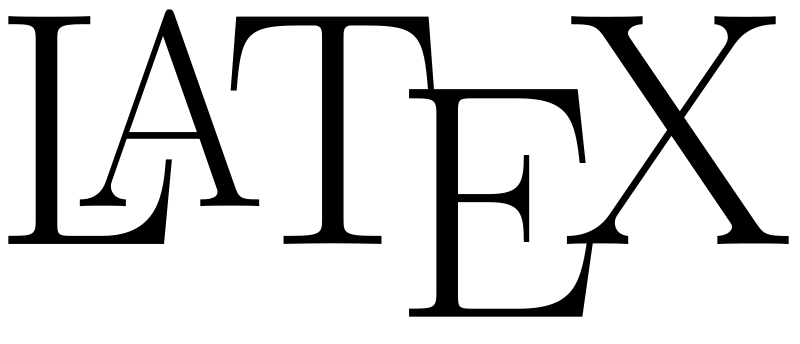
\includegraphics[width=.50\textwidth]{figure}
 
 \caption{teste DE FIGURAS}
 \label{fig:01}
\end{figure}
%%%%%%%%%%%%%%%%%%%%%%%%%%%%%%%%%%%%%%%%%%%%%%%%%%%%%%%%%%%%


\section{SEÇÃO DE COMENTÁRIOS}
\subsection{SUBSEÇÃO DE COMENTÁRIOS}
\subsubsection{SUBSUBSEÇÃO DE COMENTÁRIOS}
